\chapter{Counting and sets in OWL}
\label{ch13}

Restrictions provide a concise way to describe a class of individuals in
terms of the properties we know that describe the individuals
themselves. As we saw in the previous chapter, we can use this construct
to define notions like Vegetarian (describing someone in terms of the
type of food that they eat), to sift information from a table
(describing something according to a value of one property), and to
manage groups of people or terms (describe something based on its
membership in a group). The restrictions defined in Chapter~\ref{ch12} are
powerful methods for defining classes of individuals.

In this chapter, we see that OWL augments this capability with a full
set theory language, including intersections, unions, and complements.
These can be used to combine restrictions together (e.g., the set of
planets that go around the sun and have at least one moon) or to combine
the classes we use to define restrictions (a Vegetarian is someone who
eats food that is not Meat). This combination provides a potent system
for making very detailed descriptions of information.
OWL also includes restrictions that refer to cardinalities---that is,
referring to the number of distinct values for a particular property
some individual has. So we can describe ``the set of planets that have
at least three moons'' or ``the teams that contain more than one
all-star player.'' Reasoning with cardinalities in OWL is surprisingly
subtle. Perhaps we shouldn't be surprised that it is difficult to count
how many distinct things there are when one thing might have more than
one name (i.e., more than one URI), and we never know when someone might
tell us about a new thing we didn't know about before. These are the
main reasons why cardinality inferencing in OWL is quite conservative in
the conclusions it can draw.

\section{UNIONS AND INTERSECTIONS}

We begin with the basic logical combinations, which are familiar from
set theory. OWL provides a facility for defining new classes as unions
and intersections of previously defined classes. All set operations can
be used on any class definition at all in OWL, including named classes
and restrictions. This allows OWL to express a wide variety of
combinations of classes and conditions. The semantics for the
constructors as one would expect, matching the set operations of the
same name.

Syntactically, they use the list constructs of RDF, as follows:

\begin{lstlisting}
U1 a owl:Class ;
   owl:unionOf (ns:A ns:B...) .
I1 a owl:Class ;
   owl:intersectionOf (ns:A ns:B...) .
\end{lstlisting}

The union of two or more classes includes the members of all those
classes combined; the intersection includes the members that belong to
every one of the classes.

The intersection of two (or more) classes is a new class; this can be
represented in OWL/RDF by either naming that class (as just shown) or by
defining an anonymous class (a resource of type \texttt{owl:Class}), which is
defined to be the intersection of other classes using the property
owl:intersectionOf (likewise owl:unionOf). An anonymous class of this
sort can be used again in a model by naming using owl:equivalentClass,
as follows:

\begin{lstlisting}
bb:MajorLeagueBaseballPlayer owl:equivalentClass
   [ a owl:Class;
     owl:intersectionOf
         (bb:MajorLeagueMember bb:Player bb:BaseballEmployee)
    ] .
\end{lstlisting}

Although the semantics of intersectionOf and unionOf are
straightforward, they have a particular application to Semantic Web
modeling when used in conjunction with restrictions.

Natural language descriptions of restrictions often have a notion of
intersection built in. ``All planets orbiting the sun'' is actually the
intersection of all things that orbit the sun (hasValue restriction) and
all planets. The set of major league baseball players is the
intersection of the things that play on a major league team
(someValuesFrom restriction) and baseball players. Intersections work
just as well on restrictions as they do on named classes; we can define
these things directly using intersections:

\begin{lstlisting}
:SolarPlanet a owl:Class;
       owl:intersectionOf (
                  :Planet
                  [ a owl:Restriction; 
		    owl:onProperty :orbits;
		    owl:hasValue :TheSun]
       ) .
:MajorLeagueBaseballPlayer a owl:Class;
       owl:intersectionOf (
                  :BaseballPlayer
                  [ a owl:Restriction;
                    owl:onProperty :playsFor; 
                    owl:someValuesFrom :MajorLeagueTeam] 
       ) .
\end{lstlisting}


\begin{example}{High-Priority Candidate Questions}

In the previous chapter, we defined a class of candidate questions based
on dependencies of selected answers, and we defined priorities for the
questions themselves. We will use the set constructors to combine these
two to form a class of candidate questions of a particular priority. An
application that asks questions and records answers using this construct
would only ask high-priority questions that have been enabled by answers
given so far.

First, let's revisit the description of \texttt{SelectedAnswer} that classifies
dependent questions as
\texttt{EnabledQuestion}:

\begin{lstlisting}
q:SelectedAnswer rdfs:subClassOf
     [ a owl:Restriction;
       owl:onProperty q:enablesCandidate;
       owl:allValuesFrom q:EnabledQuestion ] .
\end{lstlisting}

We now want to define a class of questions that we are ready to ask,
based on two criteria: First, if they have been enabled by the
description above and, second, if they are high priority. This is done
with an \texttt{intersectionOf} contstruction:

\begin{lstlisting}
q:CandidateQuestion owl:equivalentClass
    [ a owl:Class;
      owl:intersectionOf
          (q:EnabledQuestion q:HighPriorityQuestion)
    ] .
\end{lstlisting}

With this description of \texttt{q:CandidateQuestion}, only questions with value
\texttt{q:High} for the property
\texttt{q:hasPriority} can become candidates.

Alternately, we could make a more relaxed description for candidate
questions that include medium-priority questions:

\begin{lstlisting}
q:CandidateQuestion owl:equivalentClass
      [ a owl:intersectionOf
           (q:EnabledQuestion
            [ a owl:unionOf
              (q:HighPriorityQuestion q:MediumPriorityQuestion) 
            ]
           )
      ] .
\end{lstlisting}
\end{example}

\subsection{Closing the world}

A key to understanding how set operations and counting works in OWL is
the impact of the \emph{Open World Assumption}. Not only does it make counting
difficult, but even the notion of set complement is subtle when you
assume that a new fact can be discovered at any time. Who's to say that
something isn't a member of a class when the very next statement might
assert that it actually is? Fortunately, there are ways in OWL to assert
that certain parts of the world are closed; in such situations,
inferences having to do with complements or counting become much
clearer.

Consider, for example, the following bit of dialogue:

\begin{quote}
\textbf{RIMBAUD:} I saw a James Dean movie last night. \\
\textbf{ROCKY:} Was it \emph{Giant}?\\
\textbf{RIMBAUD:} No.\\
\textbf{ROCKY:} Was it \emph{East of Eden}?\\
\textbf{RIMBAUD}: No.\\
\textbf{ROCKY:} James Dean only made three movies; it must have been \emph{Rebel Without a Cause}.\\
\textbf{RIMBAUD}: Yes, it was.
\end{quote}

This sort of inference relies on the fact that James Dean made only
three movies. In light of the open world assumption, how can we make
such a claim? After all, in an open world, someone could come along at
any time and tell us about a fourth James Dean movie. We will use the
example of James Dean's movies to illustrate how OWL provides a
controlled means for modeling closed aspects of the world.

\subsection{Enumerating sets with \texttt{owl:oneOf}}

In the James Dean example, it wasn't necessary that we reject the open
world assumption completely. We simply needed to know that for a
particular class (James Dean movies), all of its members are known. When
one is in a position to enumerate the members of a class, a number of
inferences can follow.

OWL allows us to enumerate the members of a class using a construct
called \texttt{owl:oneOf}, as shown here:

\begin{lstlisting}
ss:SolarPlanet rdf:type owl:Class; 
       owl:oneOf (ss:Mercury
                  ss:Venus
                  ss:Earth
                  ss:Mars
                  ss:Jupiter
                  ss:Saturn
                  ss:Uranus
                  ss:Neptune).
\end{lstlisting}

The class \texttt{SoflarPlanet} is related via the property \texttt{owl:oneOf} to a list of
the members of the class. Informally, the meaning of this is that the
class \texttt{SolarPlanet} contains these eight individuals and no others.
\texttt{owl:oneOf} places a limit on the AAA slogan. When we say that a class is
made up of exactly these items, nobody else can say that there is
another distinct item that is a member of that class. Thus, \texttt{owl:oneOf}
should be used with care and only in situations in which the definition
of the class is not likely to change---or at least not change very
often. In the case of the solar planets, this didn't change for 50
years. We can probably expect that it won't change again for quite a
while.  And even if it does, the AAA slogan still allows anyone who disagrees to publish a competing model 
that includes whatever celestial body they want. 

Although \texttt{owl:oneOf} places a limitation on the AAA slogan and Open World
Assumption, it places no limitation on the Nonunique Naming assumption.
That is, \texttt{owl:oneOf} makes no claim about whether, say, Mercury might be
the same as Venus.

When combined with \texttt{owl:someValuesFrom}, \texttt{owl:oneOf} provides a
generalization of \texttt{owl:hasValue}. Whereas \texttt{owl:hasValue} specifies a single
value that a property can take, \texttt{owl:someValuesFrom} combined with
\texttt{owl:oneOf} specifies a distinct set of values that a property can take.

\begin{challenge}{Limiting the discourse in OWL}

In the dialogue with Rimbaud, Rocky used the fact that James Dean made
only three movies to help determine what movie Rimbaud had seen. How do
we represent this in OWL?

\solution

Since James Dean has been dead for more than 50 years, it seems a sad
but safe bet that he won't be making any more movies. We can therefore
express the class of James Dean movies using \texttt{owl:oneOf} as follows:

\begin{lstlisting}
:JamesDeanMovie a owl:Class ;
           owl:oneOf (:Giant :EastOfEden :Rebel) .
\end{lstlisting}

Informally, this states that the class \texttt{JamesDeanMovie} is made up of only
\texttt{Giant}, \texttt{EastOfEden}, and \texttt{Rebel}. What is the formal meaning of \texttt{owl:oneOf}?
As usual, we define the meaning of a construct in terms of the
inferences that can be drawn from it. In the case of \texttt{owl:oneOf}, there
are a number of inferences that we can draw.

First, we can infer that each instance listed in \texttt{owl:oneOf} is indeed a
member of the class. From our assertion about \texttt{JamesDeanMovie}, we can
infer that each of these things is a James Dean movie:

\begin{lstlisting}
* :Giant rdf:type :JamesDeanMovie.
* :EastOfEden rdf:type :JamesDeanMovie.
* :Rebel rdf:type :JamesDeanMovie.
\end{lstlisting}

The meaning of \texttt{owl:oneOf} goes further than simply asserting the members
of a class; it also asserts that these are the only members of this
class. In terms of inferences, this means that if we assert that some
new thing is a member of the class, then it must be \texttt{owl:sameAs} one of
the members listed in the \texttt{owl:oneOf} list. In our James Dean example, if
someone were to introduce a new member of the class---say:

\begin{lstlisting}
:RimbaudsMovie rdf:type :JamesDeanMovie.
\end{lstlisting}

then we can infer that \texttt{RimbaudsMovie} must be \texttt{owl:sameAs} one of the other movies
already mentioned.
\end{challenge}

This inference differs from the inferences that we have seen so far. Up
to this point, we were able to express inferences in terms of new
triples that can be inferred. In this case, the inference tells us that
some triple from a small set holds, but we don't know which one. We
can't assert any new triples, and we can't respond to a query any
differently.

How do we turn this kind of inference into something from which we
assert a triple? If we compare where we are now with the conversation
between Rocky and Rimbaud, we are right at the point where Rocky has
heard from Rimbaud that he saw a James Dean movie. Rocky doesn't know
which movie he has seen, but because of his background knowledge, he
knows that it was one of three movies. How does Rocky proceed? He
eliminates candidates until he can conclude which one it is. To do this
in OWL, we must be able to say that some individual is not the same as
another.

\subsection{Differentiating individuals with \texttt{owl:differentFrom}}

There's an old joke about the three major influences on the price of a
piece of real estate: location, location, and location. The joke is, of
course, that when you promised to name three influences, any reasonable
listener expects you to give three \emph{different} influences. Because of the
non-unique naming assumption in the Semantic Web, we have to be explicit
about these things and name things that are, in fact, different from one
another. OWL provides \texttt{owl:differentFrom} for this. Its use is quite
simple: To assert that one resource is different from another requires a
single triple:

\begin{lstlisting}
ss:Earth owl:differentFrom ss:Mars .
\end{lstlisting}

Informally, this triple means that we can rely on the fact that \texttt{ss:Earth}
and \texttt{ss:Mars} refer to different resources when making arguments by
counting or by elimination. Formally, \texttt{owl:differentFrom} supports a
number of inferences when used in conjunction with other constructs like
\texttt{owl:cardinality} and \texttt{owl:oneOf}, as we shall see.

\begin{challenge}{Process of Elimination}

Use OWL to model the dialogue between Rocky and Rimbaud so that OWL can
draw the same inference that Rocky did---namely, that Rimbaud saw \emph{Rebel
Without a Cause}.

\solution

At the beginning of the dialogue, Rocky knows that the movie Rimbaud saw
was one of the three movies: \texttt{EastOfEden}, \texttt{Giant}, or \texttt{Rebel}. We have
already shown how to represent this using \texttt{owl:oneOf}. But he doesn't know
which one. He can make a guess: Perhaps it was \texttt{Giant}. If he is right, we
can simply assert that

\begin{lstlisting}
:RimbaudsMovie owl:sameAs :Giant .
\end{lstlisting}

But what if (as was the case in the dialogue) he was wrong, and Rimbaud
didn't see \emph{Giant}? We express this in OWL, using \texttt{owl:differentFrom}, as
follows:

\begin{lstlisting}
:RimbaudsMovie owl:differentFrom :Giant.
\end{lstlisting}

This narrows things down a bit, but we still don't know whether Rimbaud
saw \emph{East of Eden} or \emph{Rebel Without a Cause}. So Rocky tries again: Was the
movie \emph{East of Eden}? When the answer is negative, we have another
\texttt{owl:different} From triple:

\begin{lstlisting}
:RimbaudsMovie owl:differentFrom :EastOfEden.
\end{lstlisting}

Now we are in the position that Rocky was in at the end of the dialogue;
we know that there are just three James Dean movies, and we know that
Rimbaud did not see \emph{Giant} or \emph{East of Eden}. Just as Rocky was able to
conclude that Rimbaud saw \emph{Rebel Without a Cause}, the semantics of
\texttt{owl:oneOf} and \texttt{owl:differentFrom} allow us to infer that

\begin{lstlisting}
:RimbaudsMovie owl:sameAs :Rebel.
\end{lstlisting}

We can see these assertions and the inference in Figure~\ref{fig:ch13.01}.
\end{challenge}

\begin{figure}
\centering
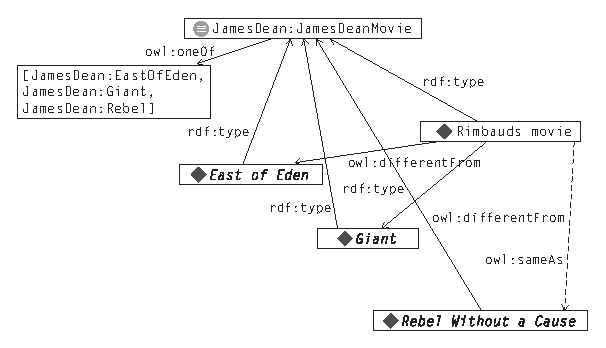
\includegraphics[width=5in]{media/ch13/f13-01.eps}
\caption{Rimbauld's movie is neither Giant nor East of Eden, so we infer that it
is Rebel Without a Cause.}
\label{fig:ch13.01}
\end{figure}



\section{Differentiating Multiple Individuals}

The nonunique naming assumption allowed us to use a new
resource---\texttt{RimbaudsMovie}---to stand in for an indeterminate movie. With
appropriate use of modeling constructs, we were able to get inferences
about which movie it actually was, using \texttt{owl:sameAs} to indicate the
answer. The nonunique naming assumption applies to all resources. For
instance, even though we intuitively know that \texttt{ss:Earth} and \texttt{ss:Mars} do
not refer to the same thing, we need to state that in our model. We did
this before using \texttt{owl:differentFrom}. We also want to say that \texttt{ss:Earth}
is different from \texttt{ss:Jupiter} and \texttt{ss:Venus}, \texttt{ss:Venus} is different from
\texttt{ss:Mars}, and so on.

To simplify the specification of lists of items, all of which are
different from one another, OWL provides \texttt{owl:AllDifferent} and
\texttt{owl:distinctMembers}---two constructs. Using these, we will specify that
a list of individuals is distinct from one another. The list of items is
specified as an RDF list. We specify that this list should be treated as
a set of mutually different individuals by referring to it in a triple
using \texttt{owl:distinctMembers} as a predicate. The domain of
\texttt{owl:distinctMembers} is \texttt{owl:AllDifferent}.

It is customary for the subject of an \texttt{owl:distinctMembers} triple to be a
bnode, so the
statement that all eight planets are mutually distinct would be
expressed in Turtle as

\begin{lstlisting}
[ a owl:AllDifferent;
  owl:distinctMembers (ss:Mercury
                       ss:Venus
                       ss:Earth
                       ss:Mars
                       ss:Jupiter
                       ss:Saturn
                       ss:Uranus
                       ss:Neptune)
] .
\end{lstlisting}

Formally, this is the same as asserting the 28 \texttt{owl:differentFrom}
triples, one for each pair of individuals in the list. In the case of
James Dean's movies, we can assert that the three movies are distinct in
the same way:

\begin{lstlisting}
[ a owl:AllDifferent;
  owl:distinctMembers (:EastOfEden
                       :Giant
                       :Rebel)
] .
\end{lstlisting}

The view of this bit of Turtle in terms of triples is shown in Figure~\ref{fig:ch13.02}.
The movies are referenced in an RDF list (using \texttt{rdf:first} and \texttt{rdf:rest}
to chain the entities together). For longer lists (like the planets),
the chain continues for each entity in the list.

Earlier we saw that the class \texttt{JamesDeanMovie} was defined using \texttt{owl:oneOf}
to indicate that these are the only James Dean movies in existence. Now
we have gone on to say that additionally these three movies are
distinct. It is quite common to use \texttt{owl:oneOf} and \texttt{owl:AllDifferent}
together in this way to say that a class is made up of an enumerated
list of distinct elements.


\begin{figure}
\centering
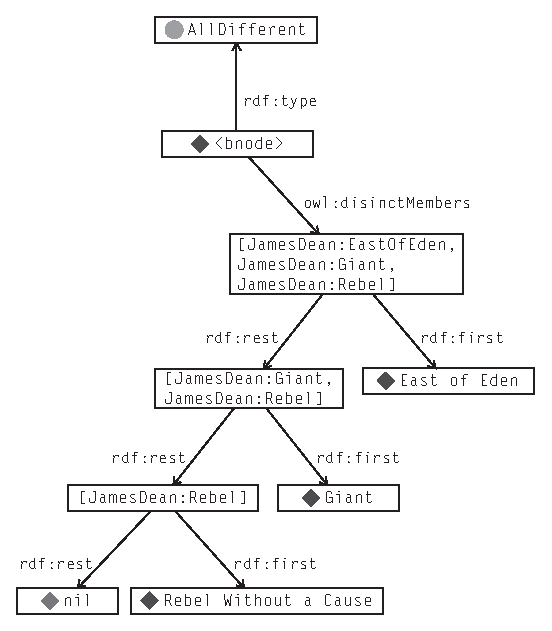
\includegraphics[width=5in]{media/ch13/f13-02.eps}
\caption{Using \texttt{owl:AllDifferent} and \texttt{owl:distinctMembers} to indicate that the
three James Dean movies are distinct. The movies are referred to in an
RDF list.
}
\label{fig:ch13.02}
\end{figure}


\section{Cardinality}

So far, we have seen restrictions that define classes based on the
presence of certain values for given properties. OWL allows a much
finer-grained way to define classes, based on the number of distinct
values a property takes. Such a restriction is called a cardinality
restriction. This seemingly simple idea turns out to have surprising
subtlety when modeling in OWL. Cardinality restrictions allow us to
express constraints on the number of individuals that can be related to
a member of the restriction class. For example, a baseball team has
exactly nine (distinct) players. A person has two (biological) parents.
Cardinality restrictions can be used to define sets of particular
interest, like the set of one-act plays or the set of books that are
printed in more than one volume.

The syntax for a cardinality restriction is similar to that for the
other restrictions we have already
seen. Here is the restriction that defines the class of things that have
exactly nine players:

\begin{lstlisting}
[ a owl:Restriction;
  owl:onProperty :hasPlayer;
  owl:cardinality 9 ]
\end{lstlisting}

Of course, instead of 9, we could have any nonnegative integer. We can
also use cardinality restrictions to specify upper and lower bounds:

\begin{lstlisting}
[ a owl:Restriction;
  owl:onProperty :hasPlayer;
  owl:minCardinality 10 ]
\end{lstlisting}

and

\begin{lstlisting}
[ a owl:Restriction;
  owl:onProperty :hasPlayer;
  owl:maxCardinality 2 ]
\end{lstlisting}

These specify the set of things that have at least 10 players and at
most 2 players, respectively. Specifying that the \texttt{owl:cardinality} is
restricted to n is the same as saying that both the \texttt{owl:minCardinality}
and \texttt{owl:maxCardinality} are restricted to the same value n. Cardinality
refers to the number of distinct values a property has; it therefore
interacts closely with the nonunique naming assumption and
\texttt{owl:differentFrom}.

The semantics of cardinality restrictions are similar to those of other
restrictions. If we can prove that
an individual has exactly (respectively at least, at most) n distinct
values for the property P, then it is a member of the corresponding
\texttt{owl:cardinality} (respectively \texttt{owl:minCardinality}, \texttt{owl:maxCardinality})
restriction. So a rugby union team (with 15 players) and a soccer team
(with 11) are both members of the restriction class with minimum
cardinality 10; a bridge team (with two players) is not, though it is a
member of the restriction class with max cardinality 2.

Similarly, if we assert that something is a member of an \texttt{owl:cardinality}
restriction, then it must have exactly n distinct values for the
property P. So if we define a baseball team to be a subclass of the
restriction class with exact cardinality 9, we can conclude that a
baseball team has exactly nine (distinct) players. Similar conclusions
follow from restrictions on minimum and maximum cardinality. We will
demonstrate the use of cardinality restrictions through a series of
challenge problems based on the James Dean example.

\begin{challenge}{Counting to three in OWL}
\label{chal:count3}
Rocky and Rimbaud continue their conversation.

\begin{quote}
\textbf{RIMBAUD:} Do you own any James Dean movies? \\
\textbf{ROCKY:} They are the only ones I own. \\
\textbf{RIMBAUD:} Then I guess you don't own very many movies! No more than three.\\
\end{quote}

Model these facts in OWL so that Rimbaud's conclusion follows from the
OWL semantics.

\solution

First we model Rocky's statement that he owns only James Dean movies. We
will need a property called
\texttt{ownsMovie} to indicate that someone owns a movie:

\begin{lstlisting}
:ownsMovie a owl:ObjectProperty.
\end{lstlisting}

In OWL, we make general statements about an individual by asserting that
the individual is a member of a restriction class. So we can say that
Rocky owns only James Dean movies by using the \texttt{owl:allValuesFrom}
restriction from Chapter\ref{ch9}:

\begin{lstlisting}
:JamesDeanExclusive owl:equivalentClass
   [ a owl:Restriction ;
     owl:onProperty :ownsMovie ;
     owl:allValuesFrom :JamesDeanMovie ] .
:Rocky a :JamesDeanExclusive .
\end{lstlisting}

Rocky is a member of the class \texttt{JamesDeanExclusive}, which is the class of
things for which all the values of \texttt{ownsMovie} come from the class
\texttt{JamesDeanMovie}.

How can we model Rimbaud's conclusion? We define the class of things
that don't own many movies (where by
``not many,'' we mean at most three) as follows:

\begin{lstlisting}
:FewMovieOwner owl:equivalentClass
[ a owl:Restriction; 
  owl:onProperty:ownsMovie;
  owl:maxCardinality 3 ] .
\end{lstlisting}

Now Rimbaud's conclusion can be formulated as a triple:

\begin{lstlisting}
* :Rocky a :FewMovieOwner .
\end{lstlisting}

This triple can be inferred from the model because all the values of the
property \texttt{ownsMovie} for Rocky come from the class \texttt{JamesDeanMovie}, and
there are only three of them, and they are all distinct, so Rocky can
own at most three movies. This inference is shown in Figure\ref{fig:ch13.03}.

\end{challenge}
\begin{figure}
\centering
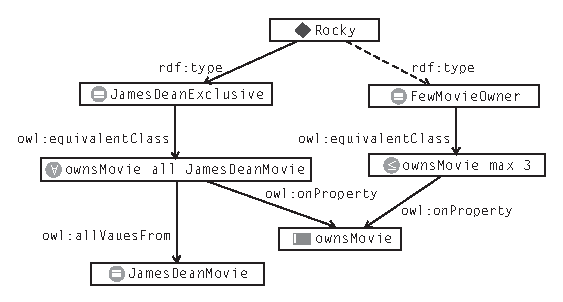
\includegraphics[width=5in]{media/ch13/f13-03.eps}
\caption{We asserted that Rocky is a \texttt{JamesDeanExclusive}; we infer that he owns
only a few movies.
}
\label{fig:ch13.03}
\end{figure}



\begin{challenge}{You can only watch three James Dean movies. } 
\label{chal:34}
Model this situation and conclusion in OWL.

\begin{quote}
\textbf{RIMBAUD:} How many movies do you own, then?  \\\
\textbf{ROCKY:} Three. \\
\textbf{RIMBAUD:} That's all of them; so you must own the one I saw last night, Rebel Without a Cause.\\
\end{quote}

\begin{figure}
\centering
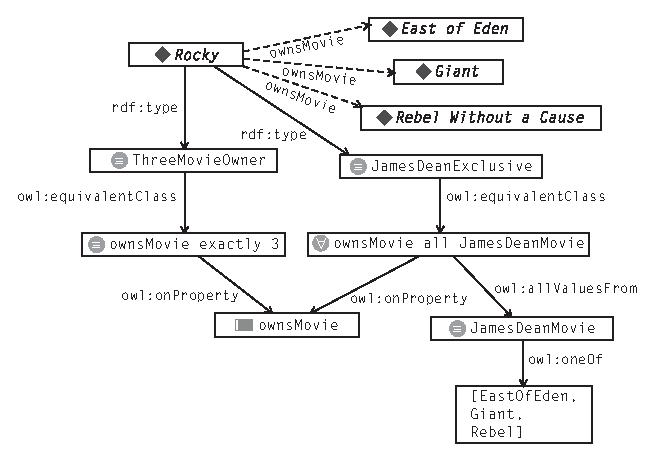
\includegraphics[width=5in]{media/ch13/f13-04.eps}
\caption{Rocky owns three movies, and he owns only James Dean movies, so he must
own each of them.}
\label{fig:ch13.04}
\end{figure}


\solution

We assert that Rocky owns exactly three movies by asserting that he is a
member of an \texttt{owl:cardinality}

restriction class for ``the set of things that own exactly three movies'':

\begin{lstlisting}
:ThreeMovieOwner owl:equivalentClass
   [ a owl:Restriction ;
     owl:onProperty :ownsMovie ;
     owl:cardinality 3 ] .
   :Rocky a :ThreeMovieOwner .
\end{lstlisting}

Since Rocky owns exactly three distinct movies, and all of his movies
are members of \texttt{JamesDeanMovie}, and there are just three different
\texttt{JamesDeanMovies}, he must own each of them. In particular, we can infer

\begin{lstlisting}
:Rocky :ownsMovie :Rebel .
\end{lstlisting}
\end{challenge}


These assertions and inferences can be seen in Figure~\ref{fig:ch13.04}.

\subsection{Qualified cardinality (OWL 2.0)}

Cardinality restrictions in OWL allow us to say how many distinct values
a property can have for any given subject. Other restrictions tell us
about the classes of which those values can or must be members. But
these restrictions work independently of one another; we cannot say how
many values from a particular class a particular subject can have. A
simple example of qualified cardinality is a model of a hand: A hand has
five fingers, one of which is a thumb.

Qualified cardinalities may seem like a needless modeling detail, and,
in fact, a large number of
models get by quite fine without them. But models that want to take
advantage of detailed cardinality information often find themselves in
need of such detailed modeling. This happens especially when modeling
the structure of complex objects.

For example, when modeling an automobile, it might be useful to say that
a properly equipped automobile includes five tires, four of which must
be regular road-worthy tires and a fifth that is a designated spare tire
which might not have all the properties of a regular tire. Structural
models of this sort often make extensive use of qualified cardinalities.

In our James Dean example, we can make use of qualified cardinality to
say that while a movie can have any number of stars, a James Dean movie
must have exactly one star who is James Dean. This is accomplished with
a slight generalization of the form for cardinality:

\begin{lstlisting}
:JamesDeanMovie rdfs:subClassOf
    [ a owl:Restriction ;
      owl:onClass :JDPerson ;
      owl:onProperty :stars ;
      owl:qualifiedCardinality "1"^^xsd:nonNegativeInteger ] .
:JDPerson a owl:Class ;
          owl:oneOf (:JamesDean) .
\end{lstlisting}

JDPerson is the singleton class that includes only James Dean; the
qualified cardinality restriction looks just like a cardinality
restriction, but includes the reference (via \texttt{owl:onClass}) to
\texttt{JDPerson}. The same conditions from non-unique naming and the open world
assumption hold for qualified cardinalities as for any others; in this
example, we could infer that

\begin{lstlisting}
:EastOfEden :stars :JamesDean .
\end{lstlisting}

This is because \texttt{EastOfEden} is a James Dean movie, and hence stars
exactly one member of the class \texttt{JDPerson}. There is only one member of
that class, so \texttt{EastOfEden} must star him. The qualified cardinality
restrictions include all of the variants of normal cardinality
restrictions, that is, \texttt{owl:maxQualifiedCardinality} and
\texttt{owl:minQualifiedCardinality}.

\subsection{Small cardinality limits}

OWL provides the facility to use any natural number as a cardinality. We
have seen how this provides an inference engine with the information
needed to determine membership in a class based on counting the number
of distinct individuals that satisfy some condition. The particular
restrictions of cardinalities to the small numbers 0 and 1 have
special modeling utility.

\begin{itemize}
\item \texttt{minCardinality 1}: The restriction of the \texttt{minCardinality} to 1 indicates
the set of individuals for which some value for the specified property
is required. The Restriction \texttt{onProperty ownsMovie minCardinality 1}
explicitly specifies the set of individuals who own at least one movie.

\item \texttt{maxCardinality 1}: The restriction of \texttt{maxCardinalilty} to 1 specifies that
a value is unique (but need not exist). The restriction \texttt{onProperty
ownsMovie maxCardinality 1} explicitly specifies the set of individuals
who own at most one movie---in other words, they have limited themselves
to a single movie.

\item \texttt{minCardinality 0}: The restriction of the \texttt{minCardinality} to 0 describes a
set of individuals for which the presence of a value for the onProperty
is optional. In the semantics of OWL, this is superfluous (since
properties are always optional anyway), but the explicit assertion that
something is optional can be useful for model readability. The
restriction \texttt{onProperty ownsMovie minCardinality 0} explicitly specifies
the set of individuals for which owning a movie is optional.

\item \texttt{maxCardinality 0}: The restriction of the \texttt{maxCardinality} to 0 indicates
the set of individuals for which no value for the specified property is
allowed. The restriction \texttt{onProperty ownsMovie maxCardinality 0}
explicitly specifies the set of individuals who own no movies.
\end{itemize}


These four special cases of cardinality are closely related.
\texttt{minCardinality 1} and \texttt{maxCardinality 0} form a partition of \texttt{minCardinality}
0; that is, \texttt{minCardinality} 1 and \texttt{maxCardinality} 0 are disjoint from one
another, they are both subclasses of \texttt{minCardinality} 0, and together
(\texttt{minCardinality 1 union maxCardinality 0}) they make up all of
\texttt{minCardinality 0} (which is equivalent to \texttt{owl:Thing}, the class of all
individuals).

\section{Set Complement}

The complement of a set is the set of all things not in that set. The
same definition applies to classes in OWL. The complement of a class is
another class whose members are all the things not in the complemented
class. Since a complement applies to a single class, we can define it
using a single triple:

\begin{lstlisting}
ex:ClassA owl:complementOf ex:ClassB .
\end{lstlisting}

Although set complements seem quite straightforward, they can easily be
misused, and OWL (like any formal system) can be quite unforgiving in
such situations.

For example, we might be tempted to say that minor league players are
the complement of major league players (asserting that there are just
these two types of players and that nobody can be both).

\texttt{bb:MinorLeaguePlayer owl:complementOf bb:MajorLeaguePlayer .
}

From this description, all of the players who are not
\texttt{bb:MajorLeaguePlayers} will be included in \texttt{bb:MinorLeaguePlayer}. However,
the complement class includes everything that is not in the referred
class, so in addition to hopeful rookies, the class \texttt{bb:MinorLeaguePlayer}
includes managers, fans, and indeed anything else in the universe, like
movies or planets.

To avoid such a situation, common practice is not to refer to
complementary classes directly. Instead, it is common practice to
combine complement with intersection:

\begin{lstlisting}
bb:MinorLeaguePlayer owl:intersectionOf
        ( [  a owl:Class;
             owl:complementOf bb:MajorLeaguePlayer ]
           bb:Player ) .
\end{lstlisting}

That is, a \texttt{MinorLeaguePlayer} is a Player who is not a \texttt{MajorLeaguePlayer}.

Thus, members of \texttt{bb:MinorLeaguePlayer} include only members of the class
\texttt{bb:Player} but does not include players that are included in
\texttt{bb:MajorLeaguePlayer}. This is much closer to the natural meaning
suggested by the name. This definition makes use of a bnode to specify
an anonymous class. There is no need to name the class that is the
complement of \texttt{bb:MajorLeaguePlayer}, so it is specified anonymously using
the bnode notation \texttt{{[} a owl:Class \ldots{} {]}}.

\begin{challenge}{Counting beyond what we know so far}
\label{chal:35}

Rocky's friend Paul joins in the discussion.

\begin{quote}
\textbf{PAUL:} Are you talking about James Dean? I love him! I have all his
movies. \\
\textbf{RIMBAUD:} But you aren't obsessive, are you? I mean, you have other
movies, too, don't you?  \\
\textbf{ROCKY:} I'm not obsessive! \\
\textbf{PAUL:} Of course, I have some movies that aren't James Dean movies. \\
\textbf{ROCKY:} You must have at least four movies then! 
\end{quote}

Model this situation and conclusion in OWL.

\solution

For this challenge, we need to have an inverse for \texttt{ownsMovie}:

\begin{lstlisting}
:ownedBy owl:inverseOf :ownsMovie .
\end{lstlisting}

We can define the class of all the movies that Paul owns as follows:

\begin{lstlisting}
:PaulsMovie a owl:Class ;
            owl:intersectionOf
              ( [ a owl:Restriction ;
	          owl:onProperty :ownedBy ;
		  owl:hasValue :Paul ]
                :Movie ) .
\end{lstlisting}

Paul says that he owns every James Dean movie---that is, every
\texttt{JamesDeanMovie} is a \texttt{PaulsMovie}
(but possibly not vice versa), so we assert

\begin{lstlisting}
:JamesDeanMovie rdfs:subClassOf :PaulsMovie .
\end{lstlisting}

Paul claims to own other movies, too. We can express that by saying

\begin{lstlisting}
:Paul a [ a owl:Restriction ;
          owl:onProperty :ownsMovie ;
          owl:someValuesFrom [ owl:complementOf :JamesDeanMovie ] 
        ] .
\end{lstlisting}

Let's look at this one in some detail.

\begin{lstlisting}
[ owl:complementOf :JamesDeanMovie ]
\end{lstlisting}

is an anonymous class (bnode) that includes everything that is not a
James Dean movie.

\begin{lstlisting}
[ a owl:Restriction ;
  owl:onProperty :ownsMovie ;
  owl:someValuesFrom [ owl:complementOf :JamesDeanMovie ]
]
\end{lstlisting}

is an anonymous class (bnode) of all the things that have some value for
owns Movie that isn't a James Dean movie. We claim that Paul is such a
thing.

Finally, we define the class of people who own four or more movies,
using \texttt{owl:minCardinality}.

\begin{lstlisting}
:ManyMovieOwner owl:equivalentClass
      [ a owl:Restriction;
        owl:onProperty :ownsMovie ;
        owl:minCardinality 4 ] .
\end{lstlisting}

Now, Paul owns all of James Dean's movies (all three of them) and at
least one that isn't a James Dean movie. That makes (at least) four in
all; so we can infer that Paul qualifies as a member of \texttt{ManyMovieOwner}.

\begin{lstlisting}
:Paul rdf:type :ManyMovieOwner .
\end{lstlisting}

These assertions and conclusion can be seen in Figure\ref{fig:ch13.05}.

\begin{figure}
\centering
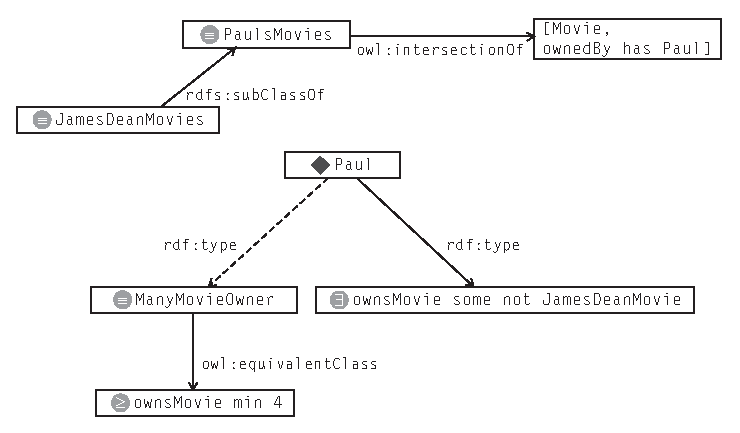
\includegraphics[width=5in]{media/ch13/f13-05.eps}
\caption{Paul owns every James Dean movie, and he owns some others, so he owns at
least four movies.
}
\label{fig:ch13.05}
\end{figure}

\end{challenge}

\section{Disjoint Sets}

We have seen how we can use \texttt{owl:complementOf} to describe the class that
includes all the individuals that are not in some class. A related idea
is that two sets have no individual in common. When this happens, we say
that the sets are disjoint, and we represent this situation in OWL using
\texttt{owl:disjointWith}, as follows:

\begin{lstlisting}
:Man owl:disjointWith :Woman .
:Meat owl:disjointWith :Fruit .
:Fish owl:disjointWith :Fowl .
\end{lstlisting}

For any members of disjoint classes, we can infer that they are
\texttt{owl:differentFrom} one another---for instance, we might assert that

\begin{lstlisting}
:Irene a:Woman .
:Ralph a:Man .
\end{lstlisting}

we can infer that

\begin{lstlisting}
:Irene owl:differentFrom :Ralph .
\end{lstlisting}

This simple idea can have powerful ramifications when combined with
other constructs in OWL, as we can see in the following challenge
problems.

\begin{challenge}{Counting in disjoint sets}
\label{chal:36}

Our moviegoers continue their conversation:

\textbf{PAUL:} I am a big movie fan. Not only do I own all the James Dean
movies, but I also have movies with Judy Garland, Tom Cruise, Dame Judi
Dench, and Antonio Banderas! \\
\textbf{ROCKY:} You must own at least seven movies! 
\textbf{PAUL:} How do you know that? \\
\textbf{ROCKY:} Because none of those people played in movies together!

Model this situation and conclusion in OWL.

\solution

How do we express, in OWL, that Paul owns a Judy Garland movie? We
assert that Paul is a member of the class of things that own Judy
Garland movies. Thus, the statements that Paul has made about the movies
he owns can be modeled in OWL using an \texttt{owl:someValuesFrom} restriction
for each one:

\begin{lstlisting}
:Paul a [ a owl:Restriction;
          owl:onProperty :ownsMovie ;
          owl:someValuesFrom :JudyGarlandMovie ] .
:Paul a  [ a owl:Restriction;
           owl:onProperty :ownsMovie ;
           owl:someValuesFrom :JudiDenchMovie ].
:Paul a [ a owl:Restriction;
          owl:onProperty :ownsMovie ;
          owl:someValuesFrom :TomCruiseMovie ] .
:Paul a [ a owl:Restriction;
          owl:onProperty :ownsMovie ;
          owl:someValuesFrom :AntonioBanderasMovie ] .
\end{lstlisting}

We can define the set of people who own seven or more movies using
\texttt{owl:minCardinality}:

\begin{lstlisting}
:SevenMovieOwner a owl:Restriction ; 
                 owl:onProperty ownsMovie ;
		 owl:minCardinality 7 .
\end{lstlisting}

How do we know that Paul is a member of this class? As Rocky points out
in the dialogue, we don't know until we know that all the sets of movies
he mentioned are disjoint. We can express this with 10 pairs of disjoint classes. or with a
single member of \texttt{owl:AllDisjointClasses}, as follows:

\begin{lstlisting}
:DisjointMovies
  rdf:type owl:AllDisjointClasses ;
  rdfs:label "Disjoint movies" ;
  owl:members (
      :AntonioBanderasMovie
      :JamesDeanMovie
      :JudiDenchMovie
      :JudyGarlandMovie
      :TomCruiseMovie
    ) ;
.
\end{lstlisting}


Now we know that Paul has three James Dean movies and at least one movie
from each of the other actors named here. Furthermore, none of these
movies appears twice, since all of the sets are disjoint. An inference
engine can confirm that Rocky is justified in counting to seven movies,
and

\begin{figure}
\centering
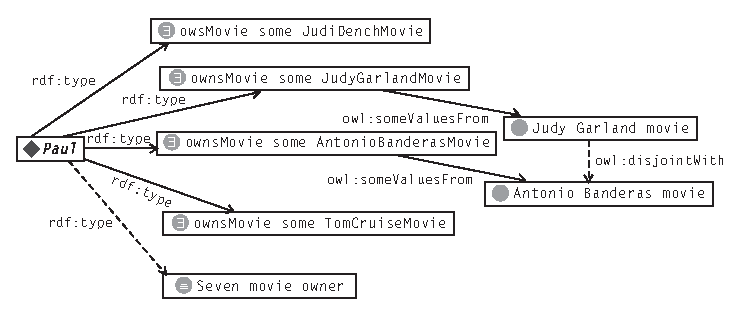
\includegraphics[width=5in]{media/ch13/f13-06.eps}
\caption{Paul owns three James Dean movies (Figure~\ref{fig:ch13.05}), plus one each from
other actors, making seven (or more) in total.}
\label{fig:ch13.06}
\end{figure}


These assertions and inferences can be seen in Figure~\ref{fig:ch13.06}.
\end{challenge}


Notice how \texttt{owl:someValuesFrom} interacts with cardinality; each
restriction of \texttt{someValuesFrom} guarantees the existence of one value for
the specified property. When these values are known to be distinct, we
can count (at least) one per \texttt{someValuesFrom} restriction.

Just as we had \texttt{owl:AllDifferent} as a way to specify that several
individuals are mutually distinct, we have \texttt{owl:AllDisjointClasses} to indicate that a set of classes is mutually disjoint, for cases like this where we kn



\section{PREREQUISITES REVISITED}

We have already explored how prerequisites can be modeled in OWL using
\texttt{owl:allValuesFrom}. At that point, we had a problem with the Open World
Assumption---namely, how can we tell that all prerequisites have been
satisfied if we have to assume that someone can come along and set new
prerequisites at any time? We'll use prerequisites to demonstrate a
number of ways we can close the world.

As a reminder from Chapter\ref{ch12}, we modeled the fact that something that
has all its prerequisites satisfied (i.e., selected) is an
EnabledQuestion as follows:

\begin{lstlisting}
q:hasPrerequisite a owl:ObjectProperty .
[ a owl:Restriction ;
  owl:onProperty hasPrerequisite ;
  owl:allValuesFrom q:SelectedAnswer ] 
 rdfs:subClassOf q:EnabledQuestion .
\end{lstlisting}

Remember that in this case, the restriction is a subclass of the named class, \texttt{EnabledQuestion}.
If something satisfies the restriction (all its values are members of
\texttt{SelectedAnswer}), then it is also a member of \texttt{EnabledQuestion}.

\subsection{No prerequisites}

Let's start with the simple situation in which we know that there are no
prerequisites at all. If something has no prerequisites, then there are
no conditions to be checked, so it should be an \texttt{EnabledQuestion}. How can
we know that something has no prerequisites?

We can assert the number of distinct values that an individual has for
some property by using the
cardinality restrictions. In particular, if we say that

\begin{lstlisting}
c:WhatProblem a [ a owl:Restriction ;
                  owl:onProperty q:hasPrerequisite ;
                  owl:cardinality 0] .
\end{lstlisting}

Then we know that there are no triples of the form

\begin{lstlisting}
c:WhatProblem q:hasPrerequisite ? .
\end{lstlisting}

That is, \texttt{WhatProblem} has no prerequisites. Therefore it satisfies the
restriction

\begin{lstlisting}
c:WhatProblem a [ a owl:Restriction ;
                  owl:onProperty hasPrerequisite ;
		  owl:allValuesFrom q:SelectedAnswer ] .
\end{lstlisting}

hence

\begin{lstlisting}
c:WhatProblem a q:EnabledQuestion.
\end{lstlisting}

The interpretation of \texttt{owl:allValuesFrom} in such a situation---that is,
when we know that there are no values from the indicated class (or even
no values at all!) can be a bit confusing. If there are no values at
all, how can all of them be members of some class? The correct way to
think about \texttt{owl:allValuesFrom} is as something that sets prerequisites,
regardless of the name of the restricted property. Let's take a simple
example: If a person has no children, then all of his or her children
are boys.

First we define the set of people all of whose children are boys, with
an \texttt{allValuesFrom}
restriction:

\begin{lstlisting}
:ParentOfBoysOnly owl:equivalentClass
[ a owl:Restriction ;
  owl:onProperty :hasChild ;
  owl:allValuesFrom :Boy ] .
\end{lstlisting}

How do we decide about membership in this class? Each triple with
predicate \texttt{hasChild} places a prerequisite for its subject to be a member
of the class. So the triple

\begin{lstlisting}
:ElizabethII :hasChild :Charles .
\end{lstlisting}

places a prerequisite for ElizabethII to be a member of
\texttt{ParentOfBoysOnly}---namely, that
Charles must be a Boy. In this case, the prerequisite is satisfied, since

\begin{lstlisting}
:Charles a :Boy .
\end{lstlisting}


But even though this prerequisite is satisfied, we still can't infer
that ElizabethII is a member of \texttt{ParentOfBoysOnly}. In order to make such
an inference, all prerequisites must be satisfied. Because of the Open
World Assumption, there might be more facts about Elizabeth that we
weren't
aware of, that is, there might be more prerequisites we have to satisfy.
In particular, if we come to learn that

\begin{lstlisting}
:ElizabethII :hasChild :Anne .
\end{lstlisting}

we will have a prerequisite that isn't satisfied, so we won't be able to
infer that ElizabethII is a member of ParentOfBoysOnly. The Open World
Assumption means that there might always be another prerequisite that we
didn't know about.

In general, it is difficult to infer that someone is a member of a class
like \texttt{ParentOfBoysOnly}, which is defined as an \texttt{allValuesFrom} restriction.
How can we ever know, in the face of the Open World Assumption, that all
prerequisites have been satisfied? One way is if we assert that there is
none. For instance, Elizabeth's ancestor, ElizabethI, was famous for
having died childless. We can assert this in OWL by asserting her
membership in a restriction class of cardinality 0, thus:

\begin{lstlisting}
:ElizabethI a [ a owl:Restriction ;
                owl:onProperty :hasChild ;
		owl:cardinality 0 ] .
\end{lstlisting}

Now we know that there are no prerequisites on ElizabethI, so we can
infer

\begin{lstlisting}
* :ElizabethI a :ParentOfBoysOnly .
\end{lstlisting}

We effectively used the cardinality restriction to close the world, at
least in the case of Elizabeth's children.

Many people find this result counterintuitive---that someone with no
children would have all of their children be boys. This conclusion is
much more intuitive if you think of \texttt{owl:allValuesFrom} as working with
prerequisites; it is intuitive to say that something that has no
prerequisites is satisfied. In the semantics of OWL, this is the
appropriate interpretation of \texttt{owl:allValuesFrom}.

\subsection{Counting prerequisites}

Another way to determine that something has satisfied all of its
prerequisites is to count how many of them there are. Just as we have
done with counting James Dean movies, we can count prerequisites.
Suppose we know that something has exactly one prerequisite:

\begin{lstlisting}
c:TvSymptom a [ a owl:Restriction ;
                owl:onProperty hasPrerequisite ;
                owl:cardinality 1 ] .
\end{lstlisting}

and that, furthermore, we actually know one prerequisite, and its type:

\begin{lstlisting}
c:TvSymptom q:hasPrerequisite d:STV .
d:STV a q:SelectedAnswer .
\end{lstlisting}

We know that one of the prerequisites is a member of the class
\texttt{q:SelectedAnswer}. We also know that there aren't any others (since the
cardinality says there is just one of them). So we know that all of the
prerequisites are members of the class \texttt{q:SelectedAnswer}:

\begin{lstlisting}
c:TVSymptom a [ a owl:Restriction ;
                owl:onProperty hasPrerequisite ;
                owl:allValuesFrom q:SelectedAnswer ] .
\end{lstlisting}

Just as in the James Dean examples, we can make inferences from larger
counts if we know that all the entities are different. If we know, for
example, that

\begin{lstlisting}
c:TVTurnedOn a [ a owl:Restriction ;
                 owl:onProperty hasPrerequisite ;
		 owl:cardinality 2 ] .
c:TVTurnedOn q:hasPrerequisite c:TVSnothing .
c:TVTurnedOn q:hasPrerequisite c:STVSnosound .
c:TVSnothing owl:differentFrom c:STVSnosound .
c:TVSnothing a q:SelectedAnswer .
c:STVSnosound a q:SelectedAnswer .
\end{lstlisting}

we can infer that

\begin{lstlisting}
c:TVTurnedOn a [ a owl:Restriction ;
                 owl:onProperty hasPrerequisite ;
		 owl:allValuesFrom q:SelectedAnswer ] .
\end{lstlisting}

since there are only two prerequisites, and we know which two they are.

\subsection{Guarantees of existence}

The issue of prerequisites revealed a subtlety in the interpretation of
\texttt{owl:allValuesFrom}---namely, that the membership of an individual A in an
\texttt{allValuesFrom} restriction on property P does not guarantee that any
triple of the form

\begin{lstlisting}
A P ?.
\end{lstlisting}

exists at all. What should be the corresponding situation in the case of
\texttt{someValuesFrom}? That is, if we say that an individual A is a member of a
restriction \texttt{onProperty} P \texttt{someValuesFrom} another class C, should we
insist that there is some triple of this form?

\begin{lstlisting}
A P ?.
\end{lstlisting}

The interpretation of \texttt{someValuesFrom} is that we do know that there is a
pair of triples of the form

\begin{lstlisting}
A P X .
X rdf:type C .
\end{lstlisting}

Evidently, if we have both of these triples, then we certainly have a
triple of the desired form. That is, in contrast to \texttt{allValuesFrom},
\texttt{someValuesFrom} does guarantee that some value is given for the specified
property.

The case for \texttt{hasValue} is even more evident than that for \texttt{someValuesFrom}.
Not only does \texttt{hasValue} guarantee that there is such a triple, but it
even specifies exactly what it is. That is, if A is a member of the
restriction \texttt{onProperty} P \texttt{hasValue} X, we can infer the triple

\begin{lstlisting}
A P X .
\end{lstlisting}

\section{Contradictions}

\begin{challenge}{Contractions from disjoint classes}
\label{chal:37}

Model this situation and conclusion in OWL.

\textbf{ROCKY:} You're a Judy Garland fan? I have a couple of her movies,too!  \\
\textbf{RIMBAUD:} Wait a minute! That can't be right! You said that you own
only James Dean movies, and now you say you have a Judy Garland movie.
They weren't in any movie together!

\solution

This solution requires us to introduce a new aspect of inferencing in
OWL. The simplest form of inferencing we have seen was where we inferred
new triples based on asserted ones. With the more advanced notions
beyond RDFS-Plus, we saw how some inferences could not themselves be
represented as triples but could result in new triples when combined
with other assertions. But in this example, there are no new triples to
be inferred at all.

Rimbaud does not make any new assertions about Rocky. Instead, he brings
into question the validity of something that Rocky has asserted. In OWL
terms, we say that Rimbaud has found a \emph{contradiction} in what Rocky has
said.

In this case, the contradiction arose because Rocky has made the
following statements:

\begin{lstlisting}
:JamesDeanExclusive owl:equivalentClass
    [ a owl:Restriction ;
      owl:onProperty :ownsMovie ;
      owl:allValuesFrom :JamesDeanMovie ] .
:Rocky a JamesDeanExclusive .
:Rocky a [ a owl:Restriction ;
           owl:onProperty :ownsMovie ;
	   owl:someValuesFrom :JudyGarlandMovie ] .
:JudyGarlandMovie owl:disjointWith :JamesDeanMovie .
\end{lstlisting}

The \texttt{owl:someValuesFrom} restriction guarantees that Rocky owns some Judy
Garland movie (though we don't know which one), and the
\texttt{owl:allValuesFrom} restriction tells us that this movie must also be a
James Dean movie. Although such a movie would have undoubtedly been very
popular, unfortunately we also know from the \texttt{owl:disjointWith} triple
that there is no such movie; somewhere in this model there is a
contradiction.

\end{challenge}

These assertions are shown in Figure~\ref{fig:ch13.07}; no inferences are shown,
since the model contains a contradiction.

\begin{figure}
\centering
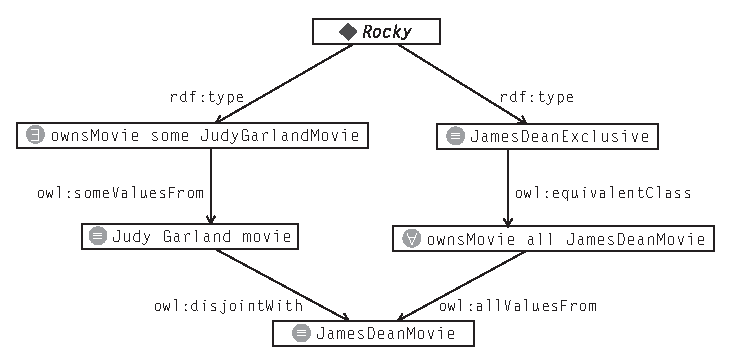
\includegraphics[width=5in]{media/ch13/f13-07.eps}
\caption{All of Rocky's films are James Dean films, but some of them are Judy
Garland films.
}
\label{fig:ch13.07}
\end{figure}



The OWL semantics can tell us that there is a contradiction in this
example, but it cannot tell us which assertion is wrong. The validity of
an assertion has nothing to do with the OWL standard or its semantics;
it has to do with the domain that is being modeled. Did Rocky lie about
owning only James Dean movies? Or is he lying now about owning Judy
Garland movies? Or, perhaps we are mistaken, and there is a Judy
Garland/James Dean collaboration out there that nobody knows about (that
is, we were mistaken when we said that these two classes were disjoint).
There is no way to know which of these statements is incorrect. But OWL
can tell us that their combination results in a contradiction.

The notion of contradiction gets to the heart of what we mean by
modeling. A model is a description of the world and can be mistaken;
that is, the model may not actually correspond to the actual state of
affairs. The tools that surround OWL models help us to determine the
nature of our models. If they are logically inconsistent, then we know
that either our model is defective or our understanding of how it
relates to the world is mistaken.

\section{Unsatisfiable Classes}

A contradiction arises when the assertions that have been made simply
cannot all be true. There is a fundamental disagreement in the asserted
statements. A similar situation can arise when we define a class in an
inconsistent way. A slight variation on the previous example shows how
this can happen. First, suppose we define the class of people who own
Judy Garland movies that Rocky claims to be a member of:

\begin{lstlisting}
:JudyGarlandMovieOwner owl:equivalentClass
   [ a owl:Restriction ;
     owl:onProperty :ownsMovie ;
     owl:someValuesFrom :JudyGarlandMovie
   ] .
\end{lstlisting}

Now, instead of claiming that Rocky is a member of both this class and
\texttt{JamesDeanExclusive}, let's define the class of such people:

\begin{lstlisting}
:JDJG owl:intersectionOf
       ( :JudyGarlandMovieOwner :JamesDeanExclusive ) .
\end{lstlisting}

Rocky has claimed to be a member of this class; this claim led to a
contradiction.

We can define this class without asserting that Rocky is a member of it.
Although this does not lead to a contradiction, the same argument that
showed that Rocky cannot (consistently) be a member of this class can be
used to show that nothing can be a member of this class, or that this
class is empty. When we can prove that a class is empty, we say that the
class itself is unsatisfiable. Although a contradiction indicates that
some statement in the model is in conflict with others, an unsatisfiable
class simply means that there can be no individuals who are members of
that class. Of course, if we go on to assert that some individual is a
member of an unsatisfiable class (as Rocky did, when he claimed to be a
member of JDJG), and then the model contains a contradiction.

Figure~\ref{fig:ch13.08} shows these assertions and the conclusions that follow. JDJG
is a subclass of both
\texttt{JudyGarlandMovieOwner} and \texttt{JamesDeanExclusive}, since it is defined as the
intersection of these two classes. But it is also inferred to be
subclass of \texttt{owl:Nothing}. This indicates in OWL that it can have no
members, since \texttt{owl:Nothing} is the class that corresponds to the empty
set.

\subsection{Propagation of unsatisfiable classes}

Once a model contains an unsatisfiable class, it is easy for other class
definitions to be unsatisfiable as well. Here are a few of the simpler
ways in which this can happen:

\begin{itemize}
\item \textbf{subclass:} A subclass of an unsatisfiable class is itself unsatisfiable.
If the subclass could (without contradiction) have an individual member,
then so could the superclass.

\item \textbf{someValuesFrom:} A restriction (on any property) with \texttt{owl:someValuesFrom}
an unsatisfiable
class is itself unsatisfiable, since \texttt{owl:someValuesFrom} requires that
there be some value that the property can indicate.

\item \textbf{domain and range:} If a property has an unsatisfiable domain or range,
then the property becomes basically unusable. Any \texttt{someValuesFrom}
restriction on that property is unsatisfiable. If any triple is asserted
using that property as predicate, then the model results in a
contradiction.

\item \textbf{intersection of disjoints}: The \texttt{owl:intersectionOf} two disjoint classes
is unsatisfiable. The intersection of any class with an unsatisfiable
class is unsatisfiable.
\end{itemize}


\begin{figure}
\centering
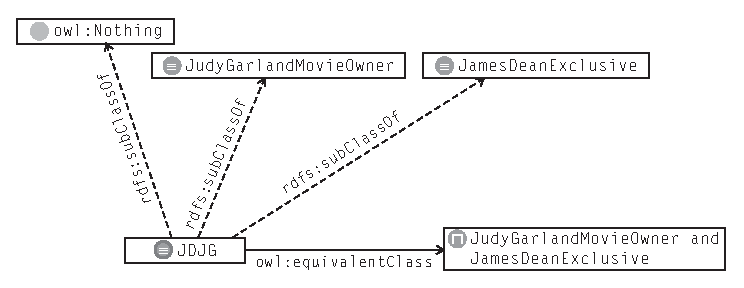
\includegraphics[width=5in]{media/ch13/f13-08.eps}
\caption{JDJG is the intersection of people who only own James Dean movies and
people who own Judy Garland movies.}
\label{fig:ch13.08}
\end{figure}



Some operations do not propagate unsatisfiable classes; the union of an
unsatisfiable class and another class can be satisfiable. A restriction
\texttt{owl:allValuesFrom} an unsatisfiable class can still be satisfiable (but
none of its members can have any value for the property specified by
\texttt{owl:onProperty} in the restriction).

These rules seem intuitive enough in isolation; their usefulness in
modeling comes in during analysis of
the results of an inference engine. Many inference engines will report
on unsatisfiable classes, but in the face of several such classes, it
can be difficult to tell just what is going on. Although some engines
have tools to assist the modeler in tracking this, the use of these
tools requires some understanding of how unsatisfiable classes can
arise. This short list is not exhaustive, but it covers most of the
common cases.

\section{Inferring Class Relationships}

In the previous discussion, most of the inferences we drew were about
individuals: Wenger is an Analyst, Jupiter is a Solar Planet, Kaneda is
a Star Player, or Shakespeare married Anne Hathaway. In this chapter, we
have begun to draw conclusions about classes---for example, JDJG is
nunsatisfiable. OWL allows us to draw a wide range of conclusions about
classes. We can, in some circumstances, infer that one class is a
subclass of another or that a class is the domain (or range) of a
property. There are countless possibilities for how this can happen, but
there are a few common patterns that are worth calling out. We'll return
to our descriptions of baseball teams for examples:

\begin{itemize}
\item \textbf{Intersection and subclass:} The intersection of two (or more) classes is
a subclass of each intersected class. If \texttt{AllStarBaseballTeam} is the
intersection of \texttt{AllStarTeam} and \texttt{BaseballTeam}, then it is also
\texttt{rdfs:subClassOf} each of those classes.

\item \textbf{Union and subclass:} The union of two (or more) classes is a superclass
of each united class.
If \texttt{JBallTeam} is the union of \texttt{PacificLeagueTeam} and \texttt{CentralLeagueTeam},
then \texttt{PacificLeagueTeam} and \texttt{CentralLeagueTeam} are both \texttt{rdfs:subClassOf}
JBallTeam.

\item \textbf{Complement and subclass:} Complement reverses the order of subclass. For
example, if \texttt{AllStarBaseballTeam} is a subclass of \texttt{BaseballTeam}, then the
complement of \texttt{BasefballTeam} is a subclass of the complement of
\texttt{AllStarBaseballTeam}.

\item \textbf{Subclass propagation through restriction:} The subclass relationships
propagate through
restrictions. If \texttt{AllStarBaseballTeam} is a subclass of \texttt{BaseballTeam}, then
the restriction (on any property---say, \texttt{playsFor}) \texttt{owl:allValuesFrom}
\texttt{AllStarBaseballTeam} is a subclass of the restriction (on the same
property \texttt{playsFor}) \texttt{owl:allValuesFrom} BaseballTeam. If we call the first
restriction \texttt{AllStarBaseballPlayer} and the second restriction
\texttt{BaseballPlayer} (both are reasonable names for these restrictions), then
this pattern says that \texttt{AllStarBaseballPlayer} is a subclass of
\texttt{BaseballPlayer}. The same propagation principle holds for any property
and also for \texttt{owl:someValuesFrom}. If
\texttt{AllStarBaseballTeam} is a subclass of \texttt{BaseballTeam}, then the restriction
on property \texttt{playsFor} some values from \texttt{AllStarBaseballTeam} is a subclass
of the restriction on property \texttt{playsFor} some values from \texttt{BaseballTeam}.

\item \texttt{hasValue}, \texttt{someValuesFrom}, and \texttt{subClassOf}: Propagation for \texttt{owl:has} Value
works a bit differently from the way it works for \texttt{owl:allValuesFrom} or
\texttt{owl:someValuesFrom}, since \texttt{owl:hasValue} refers to an individual, not a
class. Suppose that the individual \texttt{TokyoGiants} is a member of class
\texttt{BaseballTeam}; the restriction on property \texttt{playsFor} \texttt{owl:hasValue}
\texttt{TokyoGiants} is a subclass of the restriction on property \texttt{playsFor}
\texttt{owl:someValuesFrom} \texttt{BaseballTeam}.

\item \textbf{Relative cardinalities:} Subclass relations between cardinality
restrictions arise from the usual rules of arithmetic on whole numbers.
For example, if a \texttt{ViableBaseballTeam} must have at least nine players on
its roster (owl:minCardinality9), and a \texttt{FullBaseballTeam} has exactly 10
players on the roster (owl:cardinality10), then \texttt{FullfBaseballTeam} is a
subclass of \texttt{ViableBaseballTeam}.

\item \textbf{\texttt{owl:someValuesFrom} and \texttt{owl:minCardinality}:} If we say that something has
some value from a particular class, then we can infer that it has at least
one such value. So if \texttt{BaseballTeam} has some pitcher (i.e., \texttt{BaseballTeam}
is a subclass of the restriction \texttt{owl:onProperty} \texttt{hasPlayer}
\texttt{owl:someValuesFrom} \texttt{Pitcher}), we can infer that it has at least one
pitcher (i.e., \texttt{BaseballTeam} is a subclass of the restriction
\texttt{owl:onProperty} \texttt{hasPlayer} \texttt{owl:minCardinality} 1). Note that the same
conclusion does not hold for \texttt{owl:allValuesFrom}; in short, \texttt{someValuesFrom}
guarantees that there is some value; \texttt{allValuesFrom} makes no such
guarantee.
\end{itemize}

\begin{sidebar}{}
The ability in OWL to infer class relationships is a severe departure
from Object-Oriented modeling. In OO modeling, the class structure forms
the backbone of the model's organization. All instances are created as
members of some class, and their behavior is specified by the class
structure. Changes to the class structure have far-reaching impact on
the behavior of the system. In OWL, it is possible for the class
structure to change as more information is learned about classes or
individuals.


These aspects of OWL are not the result of whimsical decisions on the
part of the OWL designers; they are a direct
consequences of the basic assumptions about the Web---that is, the AAA
slogan, the Open World nature of the Web, and the fact that names on the
Web are not unique. A strict data model (like an object model) is useful
when there is top-down governance of the system (as is the case when
building a software system), but it doesn't work in an open, free system
like the Web. Our understanding of the structure of knowledge will
change as we discover more things--- we cannot escape that! OWL at least
provides a consistent and systematic way to understand those changes.
\end{sidebar}

The logic underlying OWL goes beyond these propagation rules and
encompasses inferences about subclasses regarding cardinalities. The
technical details of the logic are beyond the scope of this book. In
short, any class relationship that can be proven to hold, based on the
semantics of restrictions, unions, intersections, and so on, will be
inferred. The propagation patterns presented here don't cover all the
possible class relationship inferences, but they are the most common
patterns that appear in semantic models.

The ability in OWL to infer class relationships enables a style of
modeling in which subclass relationships are rarely asserted directly.
Instead, relationships between classes are described in terms
of unions, intersections, complements, and restrictions, and the
inference engine determines the class structure. If more information is
learned about a particular class or individual, then more class
structure can be inferred. Subclass relationships are asserted only in
that the members of one class are included in another.




\begin{table}
\caption{Overview of Entities in the Baseball Model}
\label{tab:ch13.1}
\begin{tabular}{|ll|}
AllStarBaseballPlayer&$\equiv$ playsFor some AllStarBaseballTeam \\
AllStarBaseballTeam&$\equiv$ BaseballTeam $\cap$ AllStarTeam \\
AllStarPlayer&$\equiv$ playsFor some AllStarTeam  \\
AllStarTeam&$\subseteq$ Employs only AllStarPlayer \\ 
BaseballPlayer&$\equiv$ playsFor some BaseballTeam  \\
BaseballTeam&$\subseteq$ Employs some BaseballPlayer \\
JBallTeam&$\equiv$ PacificLeagueTeam $\cup$ CentralLeagueTeam $\subseteq$ BaseballTeam \\
CarpPlayer &$\equiv$ playsFor hasValue Carp (the Carp is the name of the
baseball team from Hiroshima) \\
CentralLeagueTeam&$\equiv$ oneOf Carp, Giants, BayStars, Tigers, Dragons, Swallows \\
PacificLeagueTeam&$\equiv$ oneOf Lions, Hawks, Fighters, BlueWave, Buffaloes, Marines \\
Player&domain of playsFor  \\
Team&range of playsFor  \\
playsFor&inverse of Employs \\
\end{tabular}
\end{table}



The baseball model demonstrates this principle at work---we summarize
the statements about baseball players and their teams in Table~\ref{tab:ch13.1}.

In Table~\ref{tab:ch13.1}, we write $\equiv$ if the class in the left column is defined as
equivalent to the expression in the
right column, and $\subseteq$ if the class is a subclass of the expression in the
right column. Notice that the only direct subclass assertion (i.e., one
class is a subclass of another) is for \texttt{JBallTeam}, which is asserted to
be a subclass of \texttt{BaseballTeam}. All other assertions in the model either
refer to logical combinations (intersections or unions) or to
restrictions. Thus, the class tree as asserted is shown in Figure\ref{fig:ch13.09}.
We can infer a number of subclass relationships from the definitions of
the model in Table Table~\ref{tab:ch13.1} and the subclass inferencing patterns we have
seen.

\begin{itemize}
\item Since \texttt{AllStarBaseballTeam} is the intersection of \texttt{BaseballTeam} and
\texttt{AllStarTeam}, then \texttt{AllStarBaseballTeam} is a subclass of \texttt{BaseballTeam} and
\texttt{AllStarTeam}.

\item  Both \texttt{AllStarBaseballPlayer} and \texttt{AllStarPlayer} are \texttt{someValuesFrom}
restrictions
on the same property, \texttt{playsFor}, referencing \texttt{AllStarBaseballTeam} and
\texttt{AllStarTeam}, respectively. The fact that \texttt{AllStarBaseballTeam} is a
subclass of \texttt{AllfStarTeam} can be propagated, so we can infer that
\texttt{AllStarBaseballPlayer} is a subclass of \texttt{AllStarPlayer}. Similar reasoning
allows us to infer that \texttt{AllfStarBaseballPlayer} is a subclass of
\texttt{BaseballPlayer}.

\item  Since \texttt{JBallTeam} is the union of \texttt{PafcificLeagueTeam} and
\texttt{CentralLeagueTeam}, we can
conclude that \texttt{PacificLeagueTeam} and \texttt{CentralLeagueTeam} are subclasses of
\texttt{JBallTeam}.

\item Since the Hiroshima Carp is a \texttt{CentralLeague} team, it is also a
\texttt{JBallTeam} and thus a \texttt{BaseballTeam}. A \texttt{CarpPlayer} is a member of the \texttt{hasValue}
restriction on the Carp; thus, we can infer that \texttt{CarpPlayer} is a
subclass of \texttt{BaseballPlayer}.

\item The domain of \texttt{plfaysFor} is also used to make class inferences. Since
\texttt{AllStarPlayer} is
equivalent to the \texttt{someValuesFrom} restriction \texttt{onProperty} \texttt{playsFor}, any
individual member of \texttt{AllStarPlayer} \texttt{playsFor} some team. But the domain of
\texttt{playsFor} is \texttt{Player}, so that individual must also be a \texttt{Player}. We have
just shown that any \texttt{AllStarPlayer} must be a \texttt{Player}; thus, \texttt{AllStarPlayer}
is a subclass of \texttt{Player}.

\item Even the range information gets into the act; since an \texttt{AllStarTeam}
\texttt{employs} some
\texttt{AllStarPlayer}, and since \texttt{employs} is the inverse of \texttt{playsFor}, that means
that some person \texttt{playsFor} each \texttt{AllStarTeam}. But the range of \texttt{playsFor} is
\texttt{Team}, so \texttt{AllStarTeam} must be a \texttt{Team}, as well.


\end{itemize}


\begin{figure}
\centering
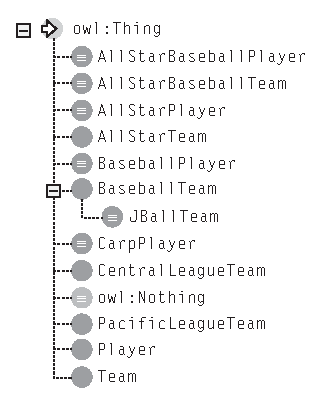
\includegraphics[width=5in]{media/ch13/f13-09.eps}
\caption{Class tree for the baseball ontology, as asserted.}
\label{fig:ch13.09}
\end{figure}



We can see the inferred class structure in Figure 12.10. Notice that
every class is involved in some class inferencing pattern so that in
contrast to the asserted model, the inferred model has considerable
depth to its class tree.

\begin{figure}
\centering
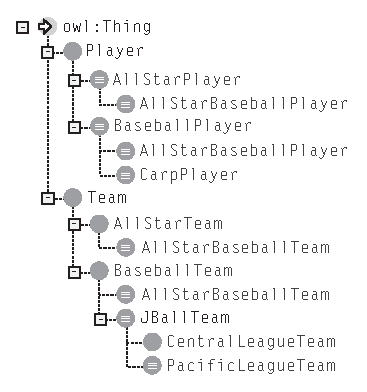
\includegraphics[width=5in]{media/ch13/f13-10.eps}
\caption{Inferred structure of the baseball model.}
\label{fig:ch13.10}
\end{figure}

\section{Reasoning with Individuals and with Classes}

From an RDF perspective, inferencing about individuals and inferencing
about classes is very similar. In both cases, new triples are added to
the model based on the triples that were asserted. From a modeling
perspective, the two kinds of reasoning are very different. One of them
draws specific conclusions about individuals in a data stream, while the
other draws general conclusions about classes of individuals. These two
kinds of reasoning are sometimes called \emph{A-box} reasoning (for individuals)
and \emph{T-box} reasoning (for classes). The curious names A-box, for
``assertion box'', and T-box, for terminology box'', are historical and
no longer have any relevance.

The utility of reasoning about individuals in a Semantic Web context is
clear, and we have seen a number of examples of it throughout this book.
We inferred things about the wife of Shakespeare, which movies belong to
which people, and what terms are broader than others. All of these
things are examples of reasoning about an individual. Information
specified in one information source is transformed according to a model
for use in another context. Mappings from one context to the next are
specified using constructs like \texttt{rdfs:subClassOf}, \texttt{rdfs:subPropertyOf}, and
various \texttt{owl:Restrictions}. Data can then be transformed and processed
according to these models and the inferences specified in the RDFS and
OWL standards for each of them.

The utility of reasoning about classes is more subtle. It can take place
in the absence of any data at all! Class reasoning determines the
relationships between classes of individuals. It determines how data are
related in general. In advance of seeing any data about the Pacific
League, we can determine that any team in that league is a baseball
team. There is no need to process all the particular teams, or indeed
any of them. We can guarantee that this is the case. Even if new teams
join the league, we know that this will still be true. In this sense,
class reasoning is similar to a compilation of the model. Whereas
individual reasoning processes particular data items as input, Class
reasoning determines general relationships among data and records those
relationships with \texttt{rdfs:subClassOf}, \texttt{rdfs:subPropertyOf}, \texttt{rdfs:domain}, or
\texttt{rdfs:range}. Once these general relationships have been inferred,
processing of individual data can be done much more easily.

When we use individual and class reasoning together in a single system,
we have a powerful system that smoothly integrates general reasoning
with specific data transformations. This allows us to smoothly manage
information based on whatever information we come across, generic or
specific.

\section{SUMMARY}

At each level of our exposition of the Semantic Web languages from RDF
to RDFS to the various levels of OWL, we have introduced new notions of
how to understand a model. For RDF, the fundamental aspect of the model
had to do with data sharing and federation. RDF answers the question
``How do I get all the information I know about a single thing in one
place?'' For RDFS, we introduced the notion of inference, answering the
question ``Given that I know certain things about my data, what else can
I figure out?'' RDFS-Plus and the basic use of OWL gave us more
comprehensive capabilities to infer new information from old. As we move
on to the advanced features OWL, we are still working within the
paradigm of inferencing as the source of meaning of our models, but we
expand the sort of inferencing we can make to include inferences not
just about our data but also about the model itself.

Up to this point, we could, for the most part, ignore the ramifications
of the Open World Assumption of the Semantic Web. With the advanced
constructs of OWL, where we can draw conclusions based on arguments of
enumeration and elimination (as well as arguments based on properties
and types, as we did with RDFS and RDFS-Plus), the impact of the open
world becomes more apparent.

Armed with the concepts and constructs OWL from this chapter, we are now
in a position to examine some more comprehensive OWL models. We can see
how a modeler can use the constructs of OWL to describe how data from
different sources will be federated on the Semantic Web. Just as we saw
for RDFS-Plus, a model can mediate information from sources that have
not yet been examined. Advanced OWL provides more powerful and complete
ways to make this happen.

\subsection{Fundamental concepts}

The following fundamental concepts were introduced in this chapter.

owl:unionOf, owl:intersectionOf, owl:complementOf---Basic set operations
applied to classes. Each of these is used to create a new class, based
on the specified set operation applied to one or more defined classes.

Open World Assumption---This idea was introduced in Chapter 1, but
strategies for closing the world for certain purposes were introduced
here.

owl:oneOf---Specifies that a class consists just of the listed members.

owl:differentFrom---Specifies that one individual is not owl:sameAs
another. This is particularly useful when making counting arguments.

owl:disjointWith---Specifies that two classes cannot share a member.
This is often used as a sort of wholesale version of owl:differentFrom.

owl:AllDisjointClasses---Specifies that each pair in a set of classes is disjoint. 

owl:cardinality, owl:minCardinality, owl:maxCardinality---Cardinality

specifies information about the number of distinct values for some
property. Combined with owl:oneOf, owl:differentFrom, owl:disjointWith,
and so on, it can be the basis of inferences based on counting the
number of values for a property.

Contradiction---With the advanced constructs of OWL, it is possible for
a model to express a contradiction---that is, for a model to be
logically inconsistent.

Satisfiability (unsatisfiability)---With the advanced constructs of OWL,
it is possible to infer that a class can have no members, so such a
class is unsatisfiable.
